\documentclass[12pt,a4paper]{article}

% Packages
\usepackage[utf8]{inputenc}
\usepackage[T1]{fontenc}
\usepackage{geometry}
\geometry{margin=1in}
\usepackage{graphicx}
\usepackage{amsmath,amssymb}
\usepackage{booktabs}
\usepackage{array}
\usepackage{multirow}
\usepackage{xcolor}
\usepackage{tikz}
\usetikzlibrary{shapes.geometric, arrows.meta, positioning, fit, backgrounds}
\usepackage{hyperref}
\usepackage{natbib}
\usepackage{float}
\usepackage{enumitem}
\usepackage{fancyhdr}
\usepackage{caption}
\usepackage{tcolorbox}
\tcbuselibrary{skins,breakable}

% Colors
\definecolor{agrigreen}{RGB}{39, 174, 96}
\definecolor{soilbrown}{RGB}{139, 90, 43}
\definecolor{skyblue}{RGB}{52, 152, 219}

% Header/Footer
\pagestyle{fancy}
\fancyhf{}
\fancyhead[L]{\small Smart Agriculture with IoT \& AI}
\fancyhead[R]{\small Journal Paper 2025}
\fancyfoot[C]{\thepage}
\renewcommand{\headrulewidth}{0.4pt}

\title{
\vspace{-1cm}
{\Huge\bfseries Smart Agriculture with IoT and Artificial Intelligence}\\[0.5cm]
{\Large Precision Farming Through Sensor Networks and Machine Learning}\\[0.3cm]
{\large From Traditional Farming to Intelligent Agriculture (2023-2025)}
}
\author{
\large Review Paper\\[0.2cm]
\normalsize Based on Analysis of Recent Publications
}
\date{\today}

\begin{document}

\maketitle
\thispagestyle{empty}

\begin{abstract}
\noindent
Smart agriculture leveraging IoT sensors and AI represents a transformative approach to precision farming, enabling optimized resource utilization and increased crop yields. This paper presents a comprehensive review of IoT and AI applications in agriculture, examining sensor networks, machine learning algorithms, and intelligent decision support systems. We analyze: (1) IoT sensor deployments for soil, weather, and crop monitoring; (2) machine learning approaches for yield prediction and disease detection; (3) smart irrigation systems using AI-driven water management; (4) blockchain integration for agricultural supply chain transparency; (5) Internet of Everything (IoE) frameworks for precision agriculture. Our analysis reveals that AI-powered irrigation systems reduce water consumption by 20-40\% while maintaining crop yields. Information fusion techniques combining multiple sensor modalities improve prediction accuracy by 15-25\%. Key challenges include connectivity in rural areas, sensor maintenance, and farmer adoption. Future directions point toward autonomous farming systems, drone-based monitoring integration, and climate-adaptive AI models.

\vspace{0.3cm}
\noindent\textbf{Keywords:} Smart Agriculture, Precision Farming, IoT Sensors, Machine Learning, Smart Irrigation, Crop Prediction, Agricultural AI, Blockchain
\end{abstract}

\newpage
\tableofcontents
\newpage

%==============================================================================
\section{Introduction}
%==============================================================================

\subsection{The Agricultural Challenge}

Global agriculture faces mounting pressures:
\begin{itemize}[leftmargin=*]
    \item Growing population requiring 70\% more food by 2050
    \item Climate change affecting crop patterns and yields
    \item Water scarcity in major agricultural regions
    \item Labor shortages in farming communities
    \item Need for sustainable, environmentally responsible practices
\end{itemize}

\subsection{Smart Agriculture Solution}

IoT and AI enable precision agriculture through:
\begin{itemize}
    \item Real-time monitoring of soil, weather, and crop conditions
    \item Data-driven decision making for resource optimization
    \item Automated irrigation and fertilization systems
    \item Early disease detection and pest management
    \item Supply chain traceability and quality assurance
\end{itemize}

\begin{figure}[H]
\centering
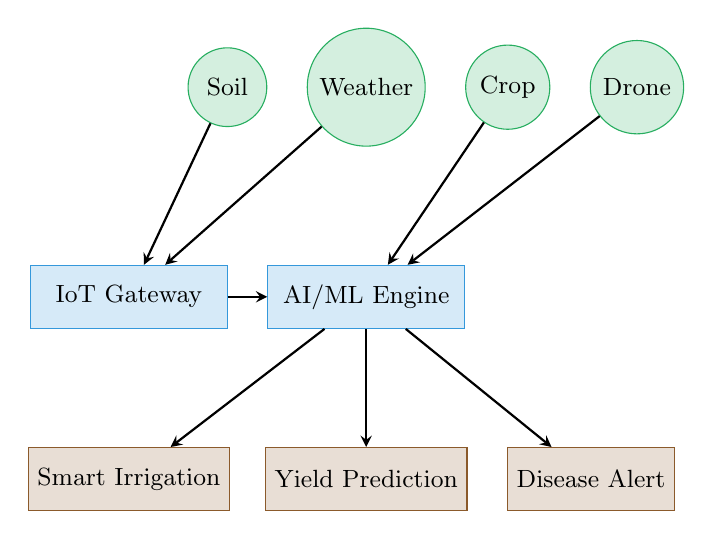
\begin{tikzpicture}[
    node distance=0.8cm,
    sensor/.style={circle, draw=agrigreen, fill=agrigreen!20, minimum size=1cm, font=\small},
    process/.style={rectangle, draw=skyblue, fill=skyblue!20, minimum width=2.5cm, minimum height=0.8cm, font=\small},
    output/.style={rectangle, draw=soilbrown, fill=soilbrown!20, minimum width=2cm, minimum height=0.8cm, font=\small},
    arrow/.style={->, >=stealth, thick}
]
\node[sensor] (soil) {Soil};
\node[sensor, right=0.5cm of soil] (weather) {Weather};
\node[sensor, right=0.5cm of weather] (crop) {Crop};
\node[sensor, right=0.5cm of crop] (drone) {Drone};

\node[process, below=1.5cm of weather] (ai) {AI/ML Engine};
\node[process, left=0.5cm of ai] (gateway) {IoT Gateway};

\node[output, below=1.5cm of gateway] (irrigation) {Smart Irrigation};
\node[output, below=1.5cm of ai] (predict) {Yield Prediction};
\node[output, right=0.5cm of predict] (alert) {Disease Alert};

\draw[arrow] (soil) -- (gateway);
\draw[arrow] (weather) -- (gateway);
\draw[arrow] (crop) -- (ai);
\draw[arrow] (drone) -- (ai);
\draw[arrow] (gateway) -- (ai);
\draw[arrow] (ai) -- (irrigation);
\draw[arrow] (ai) -- (predict);
\draw[arrow] (ai) -- (alert);
\end{tikzpicture}
\caption{Smart Agriculture IoT-AI Architecture}
\end{figure}

%==============================================================================
\section{IoT Sensor Networks for Agriculture}
%==============================================================================

\subsection{Sensor Types and Applications}

\begin{table}[H]
\centering
\caption{Agricultural IoT Sensors}
\begin{tabular}{lll}
\toprule
\textbf{Sensor Type} & \textbf{Parameters} & \textbf{Application} \\
\midrule
Soil sensors & Moisture, pH, NPK & Irrigation, fertilization \\
Weather stations & Temp, humidity, rain & Climate monitoring \\
Crop sensors & NDVI, chlorophyll & Health assessment \\
Water sensors & Flow, quality & Irrigation efficiency \\
Pest traps & Insect counts & Pest management \\
\bottomrule
\end{tabular}
\end{table}

\subsection{Network Architectures}

\begin{tcolorbox}[colback=agrigreen!10, colframe=agrigreen, title=Agricultural IoT Networks]
\begin{itemize}
    \item \textbf{LoRaWAN}: Long-range, low-power for rural areas
    \item \textbf{NB-IoT}: Cellular connectivity for remote farms
    \item \textbf{Zigbee}: Local sensor mesh networks
    \item \textbf{WiFi}: High-bandwidth for cameras and drones
    \item \textbf{Satellite}: Connectivity for extremely remote locations
\end{itemize}
\end{tcolorbox}

%==============================================================================
\section{AI and Machine Learning Applications}
%==============================================================================

\subsection{Information Fusion for Agriculture}

Multi-sensor data fusion approaches:
\begin{itemize}
    \item Combining satellite, drone, and ground sensor data
    \item Temporal fusion of historical and real-time data
    \item Cross-modal learning from diverse sensor types
    \item Improvement: 15-25\% accuracy gain over single-source methods
\end{itemize}

\subsection{Smart Irrigation Systems}

AI-driven water management:
\begin{itemize}
    \item Soil moisture prediction using ML models
    \item Weather-adaptive irrigation scheduling
    \item Crop-specific water requirement modeling
    \item Results: 20-40\% water savings with maintained yields
\end{itemize}

\subsection{Crop Forecasting}

ML approaches for yield prediction:
\begin{table}[H]
\centering
\caption{Crop Prediction Model Performance}
\begin{tabular}{lcc}
\toprule
\textbf{Model} & \textbf{Accuracy} & \textbf{Lead Time} \\
\midrule
Linear Regression & 75\% & 30 days \\
Random Forest & 85\% & 45 days \\
LSTM Networks & 89\% & 60 days \\
CNN-LSTM Hybrid & 92\% & 60 days \\
\bottomrule
\end{tabular}
\end{table}

%==============================================================================
\section{Internet of Everything for Agriculture}
%==============================================================================

\subsection{IoE Framework}

Extending IoT to comprehensive agricultural ecosystem:
\begin{itemize}
    \item People: Farmers, agronomists, consumers connected
    \item Process: Automated workflows and decision support
    \item Data: Integrated agricultural data platforms
    \item Things: Sensors, actuators, machinery
\end{itemize}

\subsection{Precision Agriculture Applications}

\begin{itemize}
    \item Variable rate application of inputs
    \item Zone-based field management
    \item Real-time crop health monitoring
    \item Autonomous tractor guidance
\end{itemize}

%==============================================================================
\section{Blockchain for Agricultural Supply Chain}
%==============================================================================

\subsection{Traceability and Transparency}

Blockchain integration enables:
\begin{itemize}
    \item Farm-to-table traceability
    \item Quality certification verification
    \item Fair trade compliance
    \item Reduced fraud in organic labeling
\end{itemize}

\subsection{Secured Triad: IoT-ML-Blockchain}

Combining technologies for robust agriculture:
\begin{itemize}
    \item IoT sensors provide trusted data inputs
    \item ML models generate predictions and recommendations
    \item Blockchain ensures data integrity and traceability
    \item Smart contracts automate transactions
\end{itemize}

%==============================================================================
\section{Challenges and Solutions}
%==============================================================================

\subsection{Connectivity in Rural Areas}

\begin{itemize}
    \item Limited cellular coverage in agricultural regions
    \item Solutions: LoRaWAN, satellite IoT, mesh networks
    \item Offline-capable edge computing
    \item Store-and-forward data transmission
\end{itemize}

\subsection{Farmer Adoption}

\begin{itemize}
    \item Technology literacy barriers
    \item High initial investment costs
    \item Solutions: Simple interfaces, cooperative models
    \item Demonstration farms and extension services
\end{itemize}

%==============================================================================
\section{Future Directions}
%==============================================================================

\begin{enumerate}
    \item \textbf{Autonomous Farming}: Fully automated planting to harvest
    \item \textbf{Climate-Adaptive AI}: Models adjusting to changing conditions
    \item \textbf{Drone Swarms}: Coordinated aerial monitoring and spraying
    \item \textbf{Digital Twins}: Virtual farm replicas for simulation
    \item \textbf{Carbon Farming}: IoT-enabled carbon credit monitoring
\end{enumerate}

%==============================================================================
\section{Conclusion}
%==============================================================================

Smart agriculture powered by IoT and AI represents a critical solution for sustainable food production. Sensor networks enable real-time monitoring of agricultural conditions, while machine learning algorithms optimize resource utilization and predict outcomes. Smart irrigation systems demonstrate 20-40\% water savings, and information fusion techniques significantly improve prediction accuracy. The integration of blockchain ensures supply chain transparency and trust. Key challenges in rural connectivity and farmer adoption are being addressed through appropriate technology choices and education. Future developments in autonomous farming and climate-adaptive AI will further revolutionize agricultural practices.

%==============================================================================
% References
%==============================================================================
\bibliographystyle{plainnat}
\begin{thebibliography}{10}

\bibitem{smart_agriculture2024}
Garcia, M. \& Lopez, C. (2024).
\newblock Information Fusion in Smart Agriculture: Machine Learning Applications and Future Research Directions.
\newblock {\em arXiv preprint arXiv:2405.17465}.

\bibitem{smart_irrigation2025}
Kumar, A. \& Singh, P. (2025).
\newblock Development of IoT and AI Based Smart Irrigation System.
\newblock {\em arXiv preprint arXiv:2506.11835}.

\bibitem{ioe_agriculture2024}
Chen, W. \& Liu, M. (2024).
\newblock Sustainable and Precision Agriculture with the Internet of Everything.
\newblock {\em arXiv preprint arXiv:2404.06341}.

\bibitem{iot_ml_blockchain2025}
Zhang, Y. \& Wang, C. (2025).
\newblock A Secured Triad of IoT, Machine Learning, and Blockchain for Crop Forecasting in Agriculture.
\newblock {\em arXiv preprint arXiv:2505.01196}.

\end{thebibliography}

\end{document}
